% 小节：IMX219 版本的整体架构图和 0–12 步时序（由 tools/rpi3_camera_arch_svg.py、
% tools/rpi3_camera_steps_svg.py 生成的 SVG 转成 PDF，放在 figure/）。
\subsection{全景：IMX219 的五层架构与取帧的 13 个步骤}
\label{sec:cam-overview}

前面各小节以 OV5647 为例，一层一层地讲。换成 Camera v2 的 IMX219 以后，只有传感器驱动这一层变了（\file{imx219.c}：CCI 地址 \code{0x10}，芯片 ID \code{0x0219}，
640$\times$480 RAW10、RGGB，\code{warmup\_frames} = 5），\file{unicam.c}、DMA 槽和 \code{/dev/video0} 的接口都不变。
本小节用两张大图把整条路径放在一起看：图~\ref{fig:cam-arch-imx219} 是静态的分层结构，图~\ref{fig:cam-steps-1}～\ref{fig:cam-steps-6} 是一次
\code{camserver} 从加载模块到关闭设备的动态过程，按 0–12 步排列。

\begin{sidewaysfigure}
  \centering
  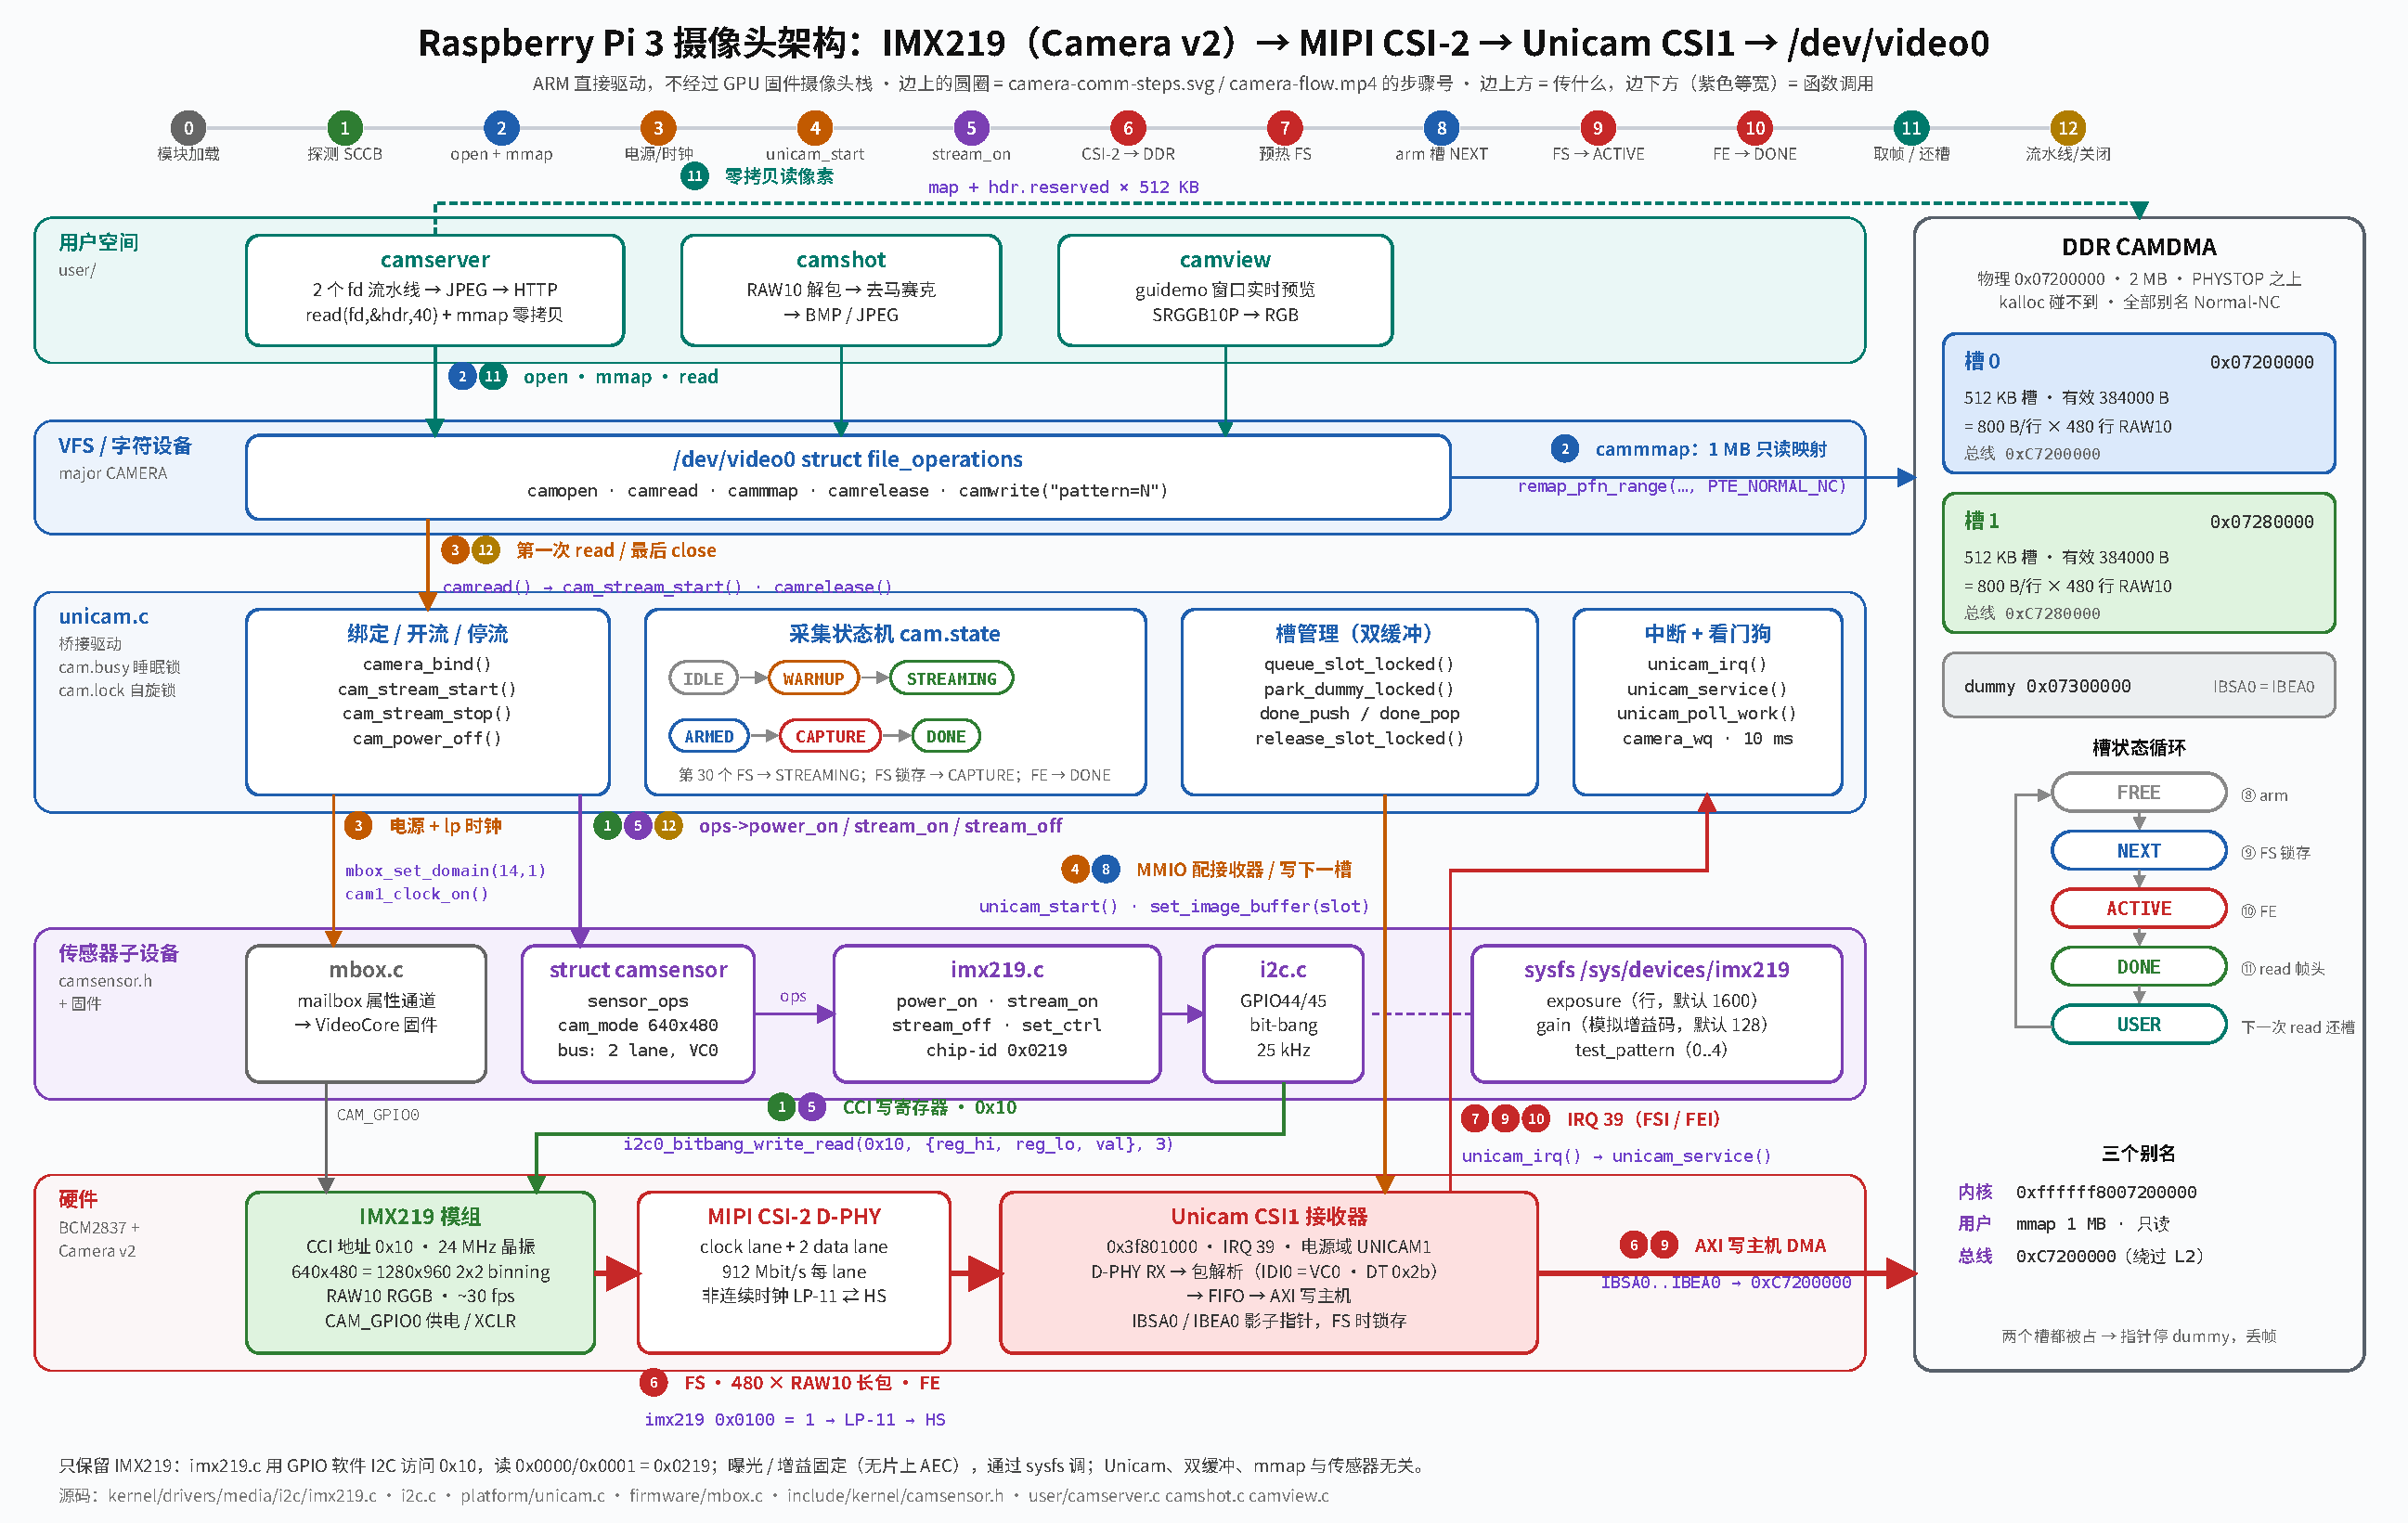
\includegraphics[width=\linewidth]{figure/camera-arch-imx219.pdf}
  \caption{IMX219 摄像头的五层架构：用户程序、\code{/dev/video0} 字符设备、\file{unicam.c} 桥接驱动（含槽管理和帧状态机）、
    传感器驱动 \file{imx219.c} 与总线（mailbox、GPIO44/45 软件 I$^2$C），以及硬件（IMX219、CSI-2 D-PHY、Unicam、DDR 里的 \code{CAMDMA}）。
    每条边上方写“做什么”，下方写调用的函数；底部的步骤条对应图~\ref{fig:cam-steps-1}～\ref{fig:cam-steps-6} 的 0–12 步}
  \label{fig:cam-arch-imx219}
\end{sidewaysfigure}

每一步画成一张卡片：标题说这一步做什么，左上角注明运行的上下文和持有的锁；中间是一条小时序图，泳道从左到右是
\code{camserver}、\file{unicam.c}、\file{imx219.c} 与 \file{i2c.c}、Unicam、IMX219 模组和 DDR，箭头上方写“做什么”，下方写实际调用；
下面是这一步涉及的寄存器位域、与 Linux 对应做法的比较，以及这一步在串口上打印的日志。
第 7–10 步就是 \ref{sec:cam-state} 小节帧状态机里的预热、排槽、FS 锁存和 FE 完成。

\newcommand{\camsteps}[3]{%
  \begin{figure}[p]
    \centering
    \includegraphics[width=\linewidth, height=0.86\textheight, keepaspectratio, page=#1]{figure/camera-comm-steps.pdf}
    \caption{IMX219 取帧的通信步骤（#1/6）：#2}
    \label{#3}
  \end{figure}}

\camsteps{1}{总览条，第 0 步模块加载、第 1 步启动探测（CCI 读芯片 ID \code{0x0219}）}{fig:cam-steps-1}
\camsteps{2}{第 2 步 \code{open} + \code{mmap}，第 3 步第一次 \code{read}：电源域、CAM1 时钟、传感器上电}{fig:cam-steps-2}
\camsteps{3}{第 4 步 \code{unicam\_start}（指针停在 dummy），第 5 步 \code{stream\_on}：CCI 写寄存器表、\code{MODE\_SELECT} = 1}{fig:cam-steps-3}
\camsteps{4}{第 6 步硬件：D-PHY LP-11 → HS、CSI-2 包、AXI 写 DDR；第 7 步预热数 FS}{fig:cam-steps-4}
\camsteps{5}{第 8 步 \code{cam\_grab} 排槽，第 9 步 FS 锁存并排第二个槽，第 10 步 FE 完成}{fig:cam-steps-5}
\camsteps{6}{第 11 步 40 字节帧头与零拷贝，第 12 步 \code{camserver} 流水线与最后一个 \code{close}}{fig:cam-steps-6}
